\section{Single Robot Method Comparison}
\label{sec:04_tdoaSingle}
\todo[inline]{Klingt etwas verkettet. Vielleicht geht sowas wie: "Direction Prediction on a Single Robot"?}
\todo[inline]{Hast du fuer die "single robot method" noch mehr als diese eine Messung? Ich finde es sehr gut, das an Hand einer einzelnen Messung zu zeigen. Fuer eine quantiative Aussage waere es aber auch gut, noch messungen aus anderen Richtungen zu haben, wenn du die hast (nur Tabelle, nicht noch mal diskutieren)}

For comparability of the results, one exemplary measurement is utilized
to present and analyse the \ac{TDOA} methods.
In this data set, the sound source is placed at the right front
of the robot with 4.5\si{m} distance.
This corresponds to an an angle of -33.7\si{\degree} in robot coordinates.
Some\todo{some klingt etwas informell} samples around the signal start of the received signal data
is plotted in \cref{fig:04_tdoaSignal} for all channels.
% -------------------------------------------------------------
\begin{figure}[ht]
	\centering
		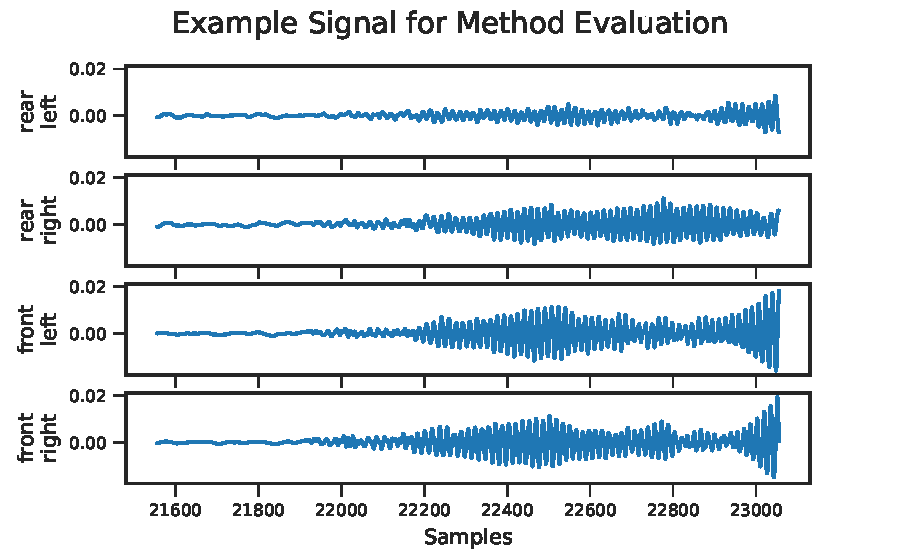
\includegraphics[]{figures/evaluation/cc_frontRight_1_signal}
	\caption{Signal start section of a whistle sound recorded from front right.}
	\label{fig:04_tdoaSignal}
\end{figure}
% -------------------------------------------------------------

As the next sections focus on the performance of the \ac{TDOA} methods,
the start index is set manually.
A frame size is defined with 256 samples and is selected around the start index for
the correlation methods as explained in \cref{sec:03_tdoa}.\todo{widerspricht sich mit dem satz davor (?) manuell vs automatisch}
For the phase method, the first frame with a size of 64 samples
is chosen where a whistle is detected in all channels.

For the sake of conciseness, throughout the following sections the correlation
function $R_{x_ax_b}$ of two signals $x_a$ and $x_b$  (\cf
\cref{chap:02_prerequisites}) is denoted as $R_{ab}$.


\subsection{Cross Correlation}
\label{subsec:04_ccSingle}
% -------------------------------------------------------------

To visualize the result of the \ac{CC}, the correlations are plotted in
\cref{fig:04_cc}. For $R_{23}$\todo{In der figure steht "R32" statt "R23"} and
$R_{13}$ a peak is clearly visible.
However, for the other \ac{CC} the problem of a low maximum peak
arises as mentioned in \cref{sec:02_cc}.
% -------------------------------------------------------------
\begin{figure}[ht]
	\centering
		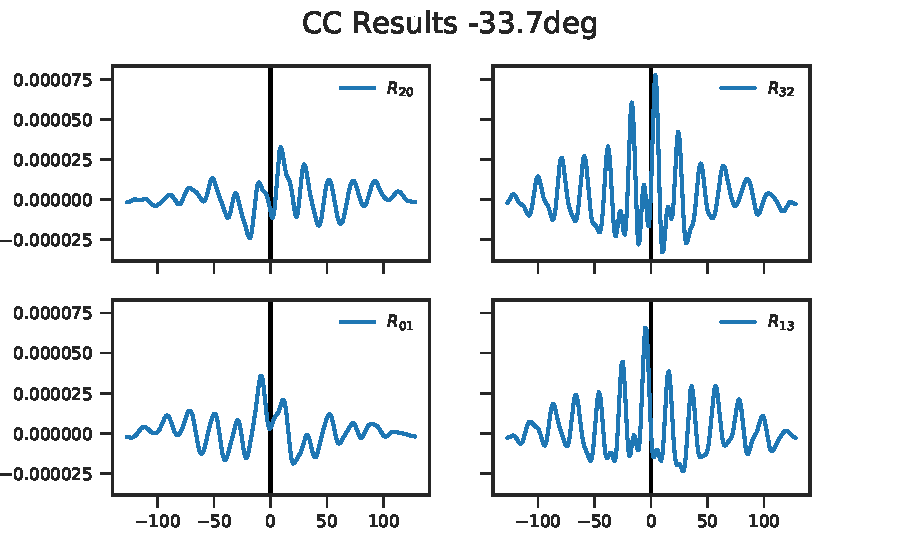
\includegraphics[]{figures/evaluation/cc_frontRight_1}
	\caption{Cross correlation results of signal from front right (-33,7\si{\degree}).}
	\label{fig:04_cc}
\end{figure}
% -------------------------------------------------------------
\btline{ht}{1.2}
\btab{|c|c|c|c|c|}
\hline
Base Channel & Next Channel & Delay & Candidate (-) & Candidate (+)\\
\hline
0 & 1 & -8.25 & -144.9 & -35.1\\
\hline
1 & 3 & -4.59 & -17.4 & 78.6\\
\hline
2 & 0 & 9.16 & -30.6 & -30.6\\
\hline
3 & 2 & 3.94 & -150.2 & -29.8\\
\hline
\etab
\et{Cross correlation delay results of signal from front right}{04_cc}
% -------------------------------------------------------------

According to the delays in \cref{tab:04_cc}, the final result of the \ac{CC}
is -26.9\si{\degree}\todo{wo kommt diese Zahl her? Finde ich die in der
Tabelle?}. Hence, the resulting prediction error is 6.8\si{\degree}.
The delay between channel 2 and 0 is larger than the maximal delay of 6.85 samples
and therefore cut to the maximum sample delay.
Besides these, the \ac{TDOA} between the channel pairs produce one appropriate
direction candidate which correctly points to the sound source.
% -------------------------------------------------------------

\subsection{Generalized Cross Correlation}
\label{subsec:04_gccSingle}
% -------------------------------------------------------------
\Cref{fig:04_gcc} presents the cross correlation result by the \ac{GCC} method of
the same signal data as in the previous section.
The subsample delays for each channel pair and their resulting direction candidates
are listed in \cref{tab:04_gcc}.
From this, a final direction of -30.0\si{\degree} is determined
resulting in an error of 3,69\si{\degree}.
It is apparent that the peaks of the \ac{GCC} are better to detect than the peaks of the
\ac{CC}.
% -------------------------------------------------------------
\begin{figure}[ht]
	\centering
		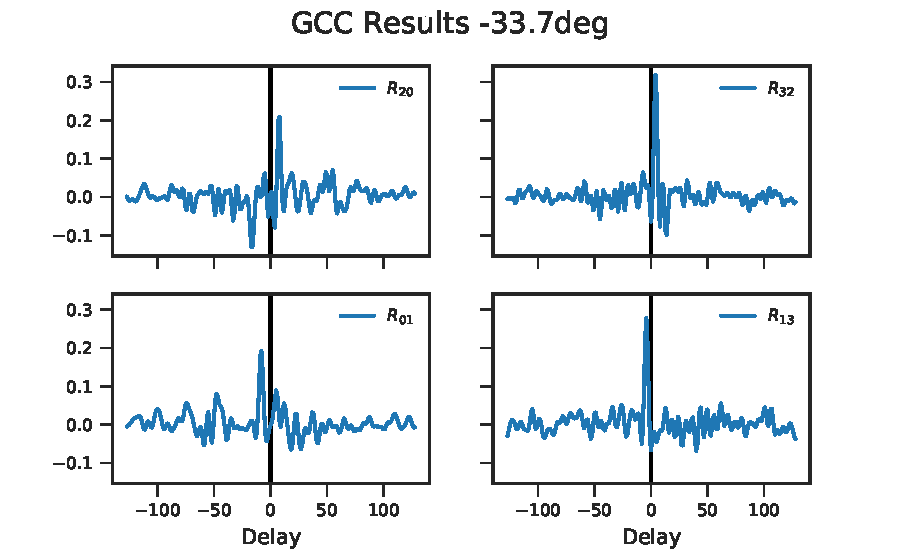
\includegraphics[]{figures/evaluation/gcc_frontRight}
	\caption{Generalized cross correlation results of signal from front right.}
	\label{fig:04_gcc}
\end{figure}
% -------------------------------------------------------------
\btline{ht}{1.2}
\btab{|c|c|c|c|c|}
\hline
Base Channel & Next Channel & Delay & Candidate (-) & Candidate (+)\\
\hline
0 & 1 & -8,28 & -144,7 & -35,3\\
\hline
1 & 3 & -4,09 & -22,8 & 84,0\\
\hline
2 & 0 & 7,60 & -30.6 & -30.6\\
\hline
3 & 2 & 4,13 & -148,7 & -31,3\\
\hline
\etab
\et{Generalized cross correlation delay results of signal from front right}{04_gcc}
% -------------------------------------------------------------
\subsection{Phase Difference}
\label{subsec:04_phaseSingle}

For detecting the source direction with phase difference, a smaller frame
size of 64 samples is defined.
In \cref{subsec:03_phase} two variants of this method were introduced that use
different strategies to identify a reference frequency. The first version uses
a static reference frequency that is fixed a-priori by the user. The second version
dynamically estimates a dominant frequency across all four channels. Hereafter,
the performance of variants is discussed.

\todo[inline]{Reihenfolge anpassen}

\subsubsection*{Dynamic Reference Frequency Selection}

First, the result of the phase difference method using a  dynamically selected
frequency are presented. As stated in the implementation chapter, the frame is
chosen where the frequencies of the maximal\todo{Du schreibst haeufiger
"maximal". Laut dictCC gibt es das aber es ist glaube ich eher unueblich}
amplitudes coincides for all channels. For the running example discussed here
this corresponds to a frequency of 2756,25\si{\hertz}.
In the upper plot of \cref{fig:04_phaseSingle}\todo{Die figure ist ganz schoen
weit weg (ich musste ein bisschen suchen)} one sees the received microphone
data which will be Hann windowed and then transformed into frequency domain by
\ac{FFT}. The resulting phases and amplitudes are listed in
\cref{tab:04_phaseSingle}.
For comprehensibility, the determined frequency information visualized by
wave signals with the detected phases and amplitudes
in the lower subplot of \cref{fig:04_phaseSingle}.
Due to the larger distance between channels 0 and 1 \todo{distance in welcher
Metric? Physical distance of the microphones? Kannst du vielleicht noch einen
satz zur klarstellung dazu schreiben.}, the phase difference information must
be neglected because the phase difference is ambiguous. Following the procedure
discussed in \todo[inline]{section ref} the resulting phase difference estimate
is -29,2\si{\degree} by combining the candidate direction -17,6\si{\degree},
-30,6\si{\degree} and -39,3\si{\degree} from channel 1, 2 and 3, respectively
(\cf \cref{tab:04_phaseDiffSingle}).
% -------------------------------------------------------------
\btline{ht}{1.2}
\btab{|c|c|c|}
\hline
Channel & Phase [\si{\deg}] & Amplitude\\
\hline
0 & -1,55 & 0,00144\\
\hline
1 & -177,7 & 0,00287\\
\hline
2 & 173,4 & 0,00279\\
\hline
3 & -75,0 & 0,00372\\
\hline
\etab
\et{Phase and amplitude of frame signals with $f_c$ = 2756,25Hz}{04_phaseSingle}
% -------------------------------------------------------------
\btline{ht}{1.2}
\btab{|c|c|c|c|c|}
\hline
Base Channel & Next Channel & Phase Difference & Candidate (-) & Candidate (+)\\
& & [\si{\deg}] & [\si{\deg}] & [\si{\deg}] \\
\hline
1 & 3 & -102,7 & -17,6 & 78,8\\
\hline
2 & 0 & 173,4 & -30,6 & -30,6\\
\hline
3 & 2 & 113,1 & -140,7 & -39,3\\
\hline
\etab
\et{Phase differences and resulting direction candidates of example data with phase method}{04_phaseDiffSingle}
% -------------------------------------------------------------
\begin{figure}[ht]
	\centering
		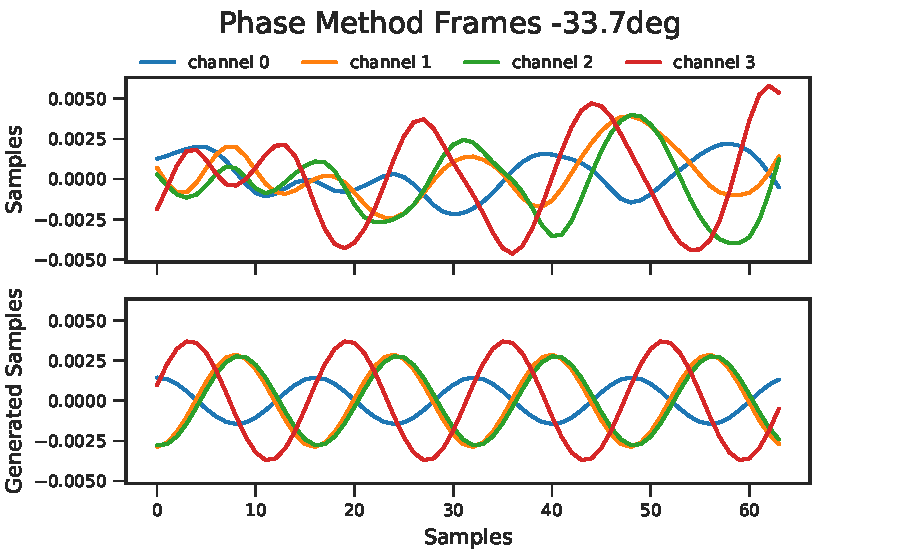
\includegraphics[]{figures/evaluation/phase_cos}
	\caption{Frames used for the direction detection by phase method.}
	\label{fig:04_phaseSingle}
\end{figure}
% -------------------------------------------------------------

\subsubsection*{Static Reference Frequency Selection}

For the phase difference method using a static frequency estimate $f_c$,
the reference frequency is set to be the first represented frequency larger
than 2600\si{\hertz}.\todo{why? Einen Satz zur Begruendung wenn es eine gibt.}
Hence, we chose $f_c = 2627,1\si{\hertz}$ with a \ac{FFT} length of 256.
Applying the phase difference method for this reference frequency, the final
direction estimate computed from the candidates listed in
\cref{tab:04_fixedFreqResult} is -29,6\si{\degree} which results in an error of
4,1\si{\degree}.
% -------------------------------------------------------------
\btline{ht}{1.2}
\btab{|c|c|c|c|c|}
\hline
Base Channel & Next Channel & Phase Difference & Candidate (-) & Candidate (+)\\
& & [\si{\deg}] & [\si{\deg}] & [\si{\deg}] \\
\hline
1 & 3 & -79,1 & -26,8 & 88,0\\
\hline
2 & 0 & 167,7 & -30,6 & -30,6\\
\hline
3 & 2 & 88,5 & -148,7 & -31,3\\
\hline
\etab
\et{Resulting candidates of phase difference method with fixed frequency
	2670,1Hz of example measurement from front right
	(-33,7\si{\degree})}{04_fixedFreqResult}
% -------------------------------------------------------------

% Configuration for Phase Method
\subsubsection*{Static Reference Frequency Value}
\label{subsubsec:04_fixedFrequencyVal}

\todo[inline]{soll das so, dass "Static Frequency Value" nicht ein unterpunt von "Static Frequency Selection" ist?}
\todo[inline]{Ich wuere fuer fc immer das wort "reference frequency" (oder
einen anderen spezifischen Term) schreiben damit man die nicht mit anderen
verwechselt.}

In order to determine the influence of the chosen reference frequency $f_c$
the phase method is tested with different frequencies in the whistle range.
For this purpose we consider a larger dataset of
\todo[inline]{num-of-measurements} measurements. In this experiment, the sound
source is recorded from eleven different positions centered around the
robot.\todo{Wenn vorhanden hier vielleicht auf eine Figure verweisen. Wenn
nicht, aber auch nicht schlimm.} This data corresponds to the measurements of
the robot with number 26 in \cref{subsec:04_labMeasurements}.

As shown in \cref{fig:04_diffFc} shows, the \ac{RMSE} is high for
frequencies smaller than 2600\si{\hertz}.
With a frequency of 2024.12\si{\hertz}, error is largest.
The result complies with the information in \cref{fig:03_maxFreq} showing that
in a whistle signal frequencies higher than 2500\si{\hertz} are dominant.
With this outcome, the fixed frequency is set to 2670,1\si{\hertz}
for further usage of the direction detection by phase method.
Limitation exists due to the ambiguity of the signal which is
content of \cref{subsubsec:03_phase}.
% -------------------------------------------------------------
\begin{figure}[ht]
	\centering
		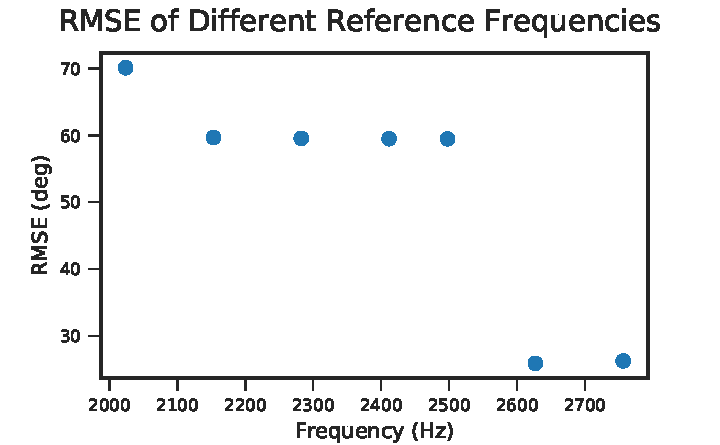
\includegraphics[]{figures/evaluation/phase_fc_rmse}
	\caption{Result of all measurements done with robot 26 to compare different
	fixed frequency values in whistle range.}
	\label{fig:04_diffFc}
\end{figure}
\todo[inline]{Errorbars?}
\todo[inline]{Ein RMSE von 30 deg scheint sehr hoch, oder nicht?}
% -------------------------------------------------------------
\subsubsection*{Frame Number}
\label{subsubsec:04_frameNumber}

Not only does the frequency play a major role for the phase method,
but also the chosen frame.
To evaluate if and how the result changes over time, the frame to
utilize is shifted by half the frame size for all measurements
of \cref{subsec:04_labMeasurements} for the robot at the center
point.
% [ 29.08029745  58.1426789   65.27548831  67.91984464  76.82890558
%   97.33976251  96.63736674 100.2203543  105.14752253  61.28179302
%   60.0017076   50.60063622  53.80158271  49.0830362   62.64453085]
In \cref{fig:04_phaseOverTime} one sees that the first channel frames with zero
shift gives the best result with a \ac{RMSE} of 29,1\si{\degree}. These results
show that the frame position has a significant influence on the prediction
accuracy of the direction detection. Therefore, an accurate signal start
detection is crucial for precise sound source localization.
% -------------------------------------------------------------
\begin{figure}[ht]
	\centering
		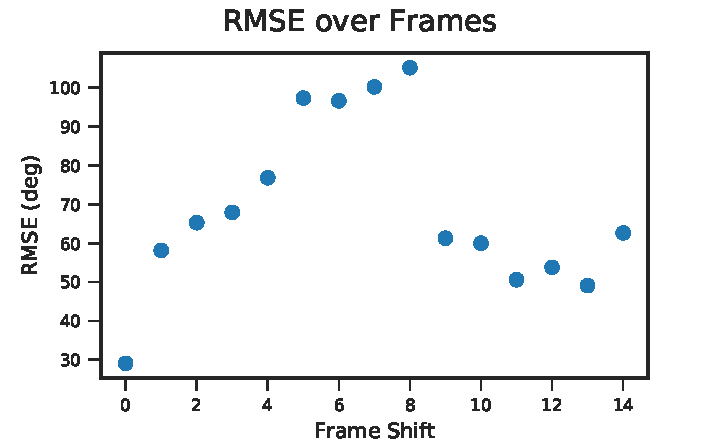
\includegraphics[]{figures/evaluation/phase_over_time}
	\caption{Changing results by shifting the frame over the
	samples. All measurements of \cref{subsec:04_labMeasurements}
	with robot nr. 26 are taken into consideration.}
	\label{fig:04_phaseOverTime}
\end{figure}
% -------------------------------------------------------------
